\documentclass[12pt]{article}
\setlength{\oddsidemargin}{0in}
\setlength{\evensidemargin}{0in}
\setlength{\textwidth}{6.5in}
\setlength{\parindent}{0in}
\setlength{\parskip}{\baselineskip}

\usepackage{amsmath,amsfonts,amssymb,graphicx,xcolor,mathtools,mathabx,siunitx}
\sisetup{tight-spacing=true}

\newcommand{\purple}[1]{{\color{purple} #1}}

\begin{document}

PHYS 374 Fall 2020\hfill Worksheet 9: Planetary Wobbles\\
\\
Name: \purple{SOLUTION} \\
\\
Please submit as a PDF on Moodle. Include any calculations made using external tools.

\hrulefill
\\
\\
Earth interacts with the Sun via a gravitational potential:
$$
U(r) = -\frac{G m_\Earth m_\Sun}{r}
$$

\begin{enumerate}
    \item Show that the equation of motion is as follows. Explain the significance of each term.
    $$
    \mu \ddot{r} = -\frac{d}{dr} \left[ \frac{\ell^2}{2 \mu r^2} -\frac{G \mu M}{r} \right]
    $$
    \item Sketch the gravitational potential, the centripetal potential, and the effective potential.
    \item Find the value $r_0$ at which $\ddot{r}=0$ and explain its significance. It's a bit messy, so be sure to double check your units!
    \item Approximate the effective potential near $r_0$ as a quadratic. Recall:
    $$
    f(x) \approx f(x_0) + f'(x_0) \; (x - x_0) + \tfrac{1}{2} f''(x) \; (x - x_0)^2 + \cdots
    \quad\quad\text{near $x_0$}
    $$
    \item Perform a change of variables $(r - r_0) \rightarrow \epsilon$. Show that the equation of motion can now be written as:
    $$
    \ddot{\epsilon} = - \omega^2 \epsilon
    $$
    \item Solve the equation of motion for $\epsilon(t)$. What is the value of $\omega$? How does this number line up with the motion of the Earth?
\end{enumerate}

The values below may be useful. Note $\ell_\Earth$ is Earth's orbital angular momentum.
\begin{align*}
    m_\Sun &= \SI{1.99e30}{\kilo\gram} &
    G &= \SI{6.67e-11}{\newton\meter^2/\kilogram^2} & \\
    m_\Earth &= \SI{5.97e24}{\kilo\gram} & 
    \ell_\Earth &= \SI{2.66e40}{\joule \second}
\end{align*}

\newpage


\purple{
The Lagrangian for Earth's orbit around the Sun in plane polar coordinates is:
$$
\mathcal{L} = \tfrac{1}{2} m_\Earth \dot{\vec{r}}^2_\Earth + \tfrac{1}{2} m_\Sun \dot{\vec{r}}^2_\Sun + \frac{G m_\Earth m_\Sun}{| \vec{r}_\Earth - \vec{r}_\Sun |}
$$
Or, in center of mass coordinates:
$$
\mathcal{L} = \underbrace{\tfrac{1}{2} M \dot{R}^2}_{\mathcal{L}_\text{cm}} + \underbrace{\tfrac{1}{2} \mu \dot{r}^2 + \frac{G \mu M}{r}}_{\mathcal{L}_\text{rel}}
$$
The equation of motion for $\vec{R}$ gives constant velocity, as we have seen. The relative motion, $\vec{r}$, is more interesting. First, swap $\vec{r}$ out for plane polar coordinates:
$$
\mathcal{L}_\text{rel} = \tfrac{1}{2} \mu \left( \dot{r}^2 + r^2 \dot{\phi}^2 \right) + \frac{G \mu M}{r}
$$
Plugging into the Euler-Lagrange equation for $\phi$ we get the constant $\ell$, representing Earth's orbital angular momentum:
$$
mr^2\dot{\phi} = \ell \quad \text{(constant)}
$$
The Euler-Lagrange equation in $r$ gives:
$$
\mu \ddot{r} = \mu r \dot{\phi}^2 + \frac{d}{dr} \left[ \frac{G \mu M}{r} \right]
$$
Using the constant $\ell$, we can rewrite the above with only $r$ (no $\phi$):
$$
\mu \ddot{r} = \frac{\ell^2}{\mu r^3} + \frac{d}{dr} \left[ \frac{G \mu M}{r} \right]
\quad\quad\rightarrow\quad\quad
\mu \ddot{r} = -\frac{d}{dr} \left[ \frac{\ell^2}{2 \mu r^2} -\frac{G \mu M}{r} \right]
$$
On the left we have the radial acceleration. This is essentially Earth's radial acceleration, since $m_\Sun \gg m_\Earth$. The two terms on the right are the centripetal potential and the gravitational potential respectively. Their sum creates a potential well as shown in the figure. 

\begin{figure}[h]
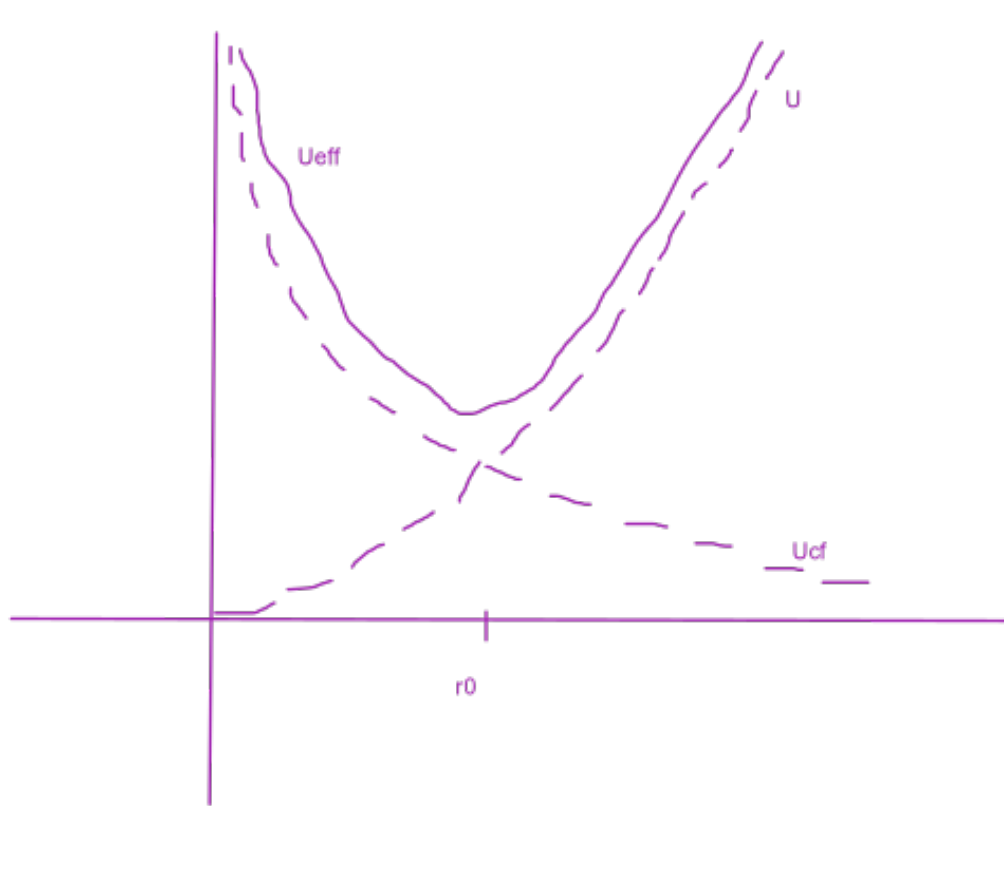
\includegraphics[width=10cm]{ueff-sketch.png}
\centering
\end{figure}

When $\mu \ddot{r}=0$, we must also have $\frac{dU_\text{eff}}{dr}=0$. At that point ($r_0$) the gravitational force and the centripetal ``force'' balance each other exactly, so $r$ is constant. Notably, $\phi$ is not constant. This is a circular orbit. We can find $r_0$:
$$
0 = \frac{d}{dr} \left[ \frac{\ell^2}{2 \mu r^2} -\frac{G \mu M}{r} \right]_{r=r_0}
\quad\quad\rightarrow\quad\quad
\frac{\ell^2}{\mu r_0^3} = \frac{G \mu M}{r_0^2}
\quad\quad\rightarrow\quad\quad
r_0 = \frac{\ell^2}{G \mu^2 M}
$$
Take a moment to convince yourself that the units here line up. The units for $G$ are at the bottom of the first page.

Next up, we expand $U_\text{eff}$ in a Taylor series around $r_0$:
$$
U_\text{eff}(r) \approx U_\text{eff}(r_0) + U_\text{eff}(r_0)\; (r - r_0) + \tfrac{1}{2} U_\text{eff} \; (r - r_0)^2
$$
This part gets a bit messy:
$$
U_\text{eff}(r_0) = 
\frac{\ell^2}{2 \mu \left(\frac{\ell^2}{G \mu^2 M}\right)^2} -\frac{G \mu M}{\frac{\ell^2}{G \mu^2 M}}
=
-\frac{G^2 \mu^3 M^2}{2 \ell^2}
$$
The next term, $U'_\text{eff}(r_0)$ is zero, since that's the whole point of $r_0$. Then finally:
$$
U''_\text{eff}(r_0) = 
3 \frac{\ell^2}{\mu \left(\frac{\ell^2}{G \mu^2 M}\right)^4} - 2 \frac{G \mu M}{\left( \frac{\ell^2}{G \mu^2 M} \right)^3}
=
\frac{G^4 \mu^7 M^4}{\ell^6}
$$
As is typical in Taylor expansions, we stop after the first non-constant term. We're trying to look at the behavior very close to $r_0$, not reconstruct the entire function. We end up with:
$$
U_\text{eff} (r) \approx -\frac{G^2 \mu^3 M^2}{2 \ell^2} + \frac{1}{2} \frac{G^4 \mu^7 M^4}{\ell^6} \; (r - r_0)^2
$$
The units check out. The signs also check out. This is a potential well with $U_\text{eff}(r_0) < 0$, then increasing on both sides ($U''_\text{eff}(r_0) > 0$). 

Plugging back into our equation of motion, we get:
$$
\mu \ddot{r} \approx -\frac{d}{dr} \left[ -\frac{G^2 \mu^3 M^2}{2 \ell^2} + \frac{1}{2} \frac{G^4 \mu^7 M^4}{\ell^6} \; (r - r_0)^2 \right]
\quad\quad\rightarrow\quad\quad
\mu \ddot{r} \approx - \frac{G^4 \mu^7 M^4}{\ell^6} \; (r - r_0)
$$
This looks an awful lot like the differential equation for a sine or cosine, but with an extra constant hanging around. One way to handle that is with a change of variables. (Another way would be to guess a solution of the form $A + B \sin \omega t$, then evaluate the derivatives to figure out $A$ and $\omega$).
$$
\epsilon = (r - r_0)
\quad\quad\text{and}\quad\quad
\ddot{\epsilon} = \ddot{r}
\quad\quad\text{so}\quad\quad
\mu \ddot{\epsilon} \approx -\frac{G^4 \mu^7 M^4}{\ell^6} \; \epsilon
$$
In other words:
$$
\ddot{\epsilon} \approx -\omega^2 \epsilon
\quad\quad\text{so}\quad\quad
\epsilon(t) \approx A \sin(\omega t + \phi_0)
\quad\quad\text{where}\quad\quad
\omega = \frac{G^2 \mu^3 M^2}{\ell^3}
$$
The constants $A$ and $\phi_0$ would be determined from initial conditions.

Plugging in some numbers, we get:
$$
\omega \approx \SI{1.99e7}{\radian/\second}
\quad\quad\text{or}\quad\quad
\omega \approx \SI{6.28}{\radian/year}
$$
The period of the perturbation lines up with the period of the orbit. In other words, perturbing a circular orbit can stretch or squish it into an ellipse. But even when that happens, it'll still be a closed orbit.

Note also: you may find it easier to plug words into Wolfram Alpha rather than typing out numbers.

\begin{figure}[h]
\includegraphics[width=12cm]{earth-orbit-wolfram.png}
\centering
\end{figure}


}

\end{document}